\section{Theorie}
  \subsection{Das Phasendiagramm}
  Bei klassischer Betrachtung liegt Wasser in einem der drei Phasen fest, flüssig oder gasförmig vor. In einem geschlossenen Raum eines abgeschlossenen Systems existieren nur
  zwei Freiheitsgrade: der Druck sowie die Temperatur können sich verändern, das Volumen ist fest. Dieser Sachverhalt lässt sich qualitativ darstellen in einem Phasendiagramm
  (hier für Wasser):
  \\
  \begin{figure}
    \centering
      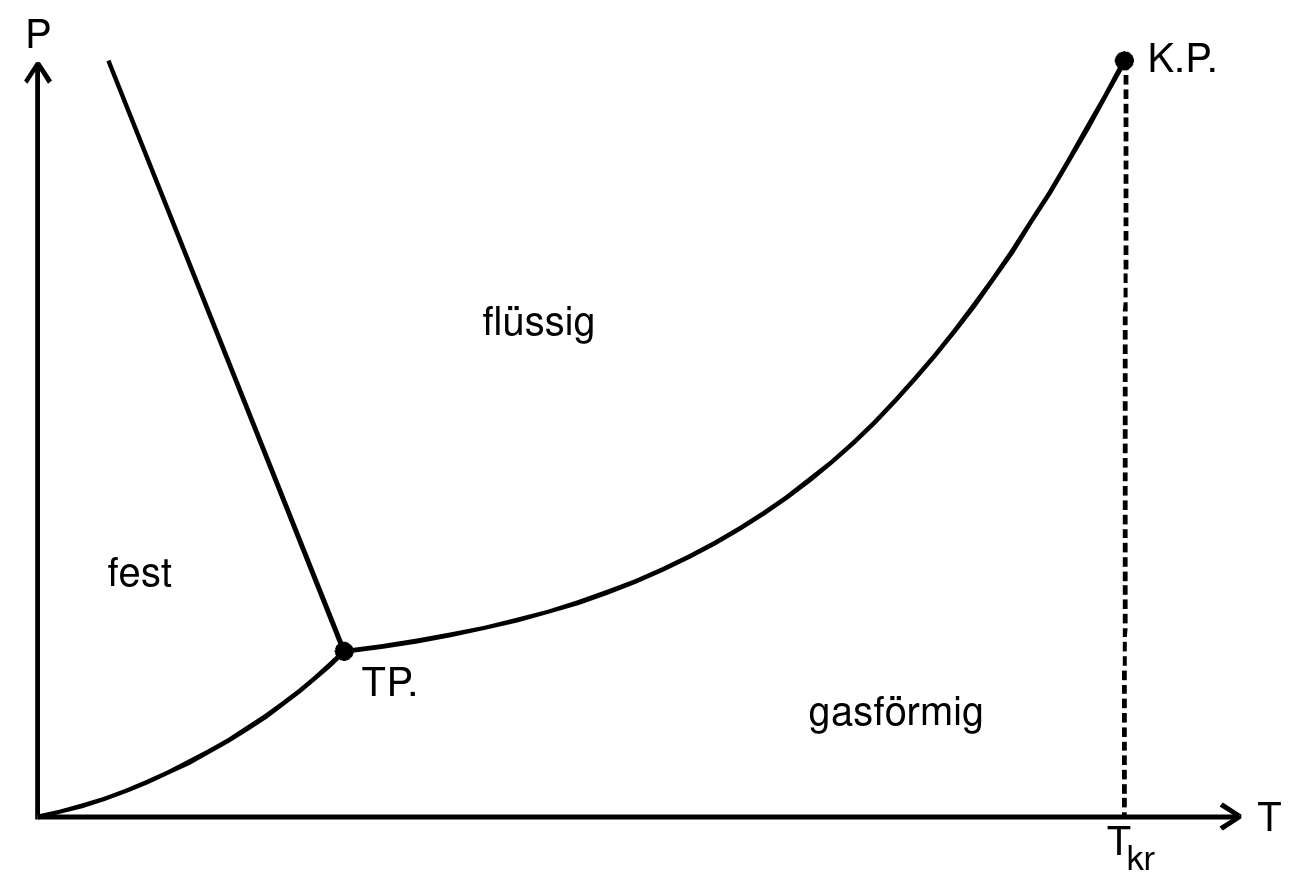
\includegraphics[scale = 0.2]{Content/phasendiagramm.png}
      \caption{ein qualitatives Phasendiagramm für Wasser.}
  \end{figure}
  \\
  \noalign
  Im Folgenden wird der Übergang von flüssig zu gasförmig betrachtet. Die beiden in obiger Abbildung eingezeichneten Punkte TP. (Tripelpunkt, hier liegen alle drei Phasen gleichzeitig vor) und K.P. (Kritischer Punkt, hier koexistieren die Phasen flüssig
  und gasförmig nebeneinander)
  begrenzen die Dampfdruckkurve. Der Verlauf dieser Kurve wird bestimmt durch die Größe der Verdampfungswärme $L$, welche für jeden Stoff verschieden ist. Sie beschreibt,
  wieviel Wärmeenergie $\increment Q$ nötig ist, um ein mol einer Flüssigkeit zu verdampfen. Diese Größe ist jedoch auch temperaturabhängig. Am kritischen Punkt der
  Dampfdruckkurve verschwindet $L$ aufgrund der Koexistenz der flüssigen und gasförmigen Phase, bei den meisten Temperaturen der Dampdruckkurve kann die Verdampfungswärme
  aber als näherungsweise konstant angesehen werden.
  \subsection{Die mikroskopischen Vorgänge während des Experiments}
  Wenn in einen abgeschlossenen und evakuierten Raum eine Flüssigkeit gebracht wird, 
\label{sec:Theorie}
